\documentclass[10pt]{article}
\usepackage[english]{babel}
\usepackage[utf8]{inputenc}


\usepackage{graphicx}
\usepackage[font=footnotesize, caption=false]{subfig}


\title{Enabling QoS Planning in Lustre}

\begin{document}

\maketitle

\section{Abstract}

Lustre introduced Quality of Service (QoS) settings in version 2.4 by extending the Network Request Scheduler (NRS) with a Token Bucket Filter (TBF) strategy.
The extension allows administrators to set QoS based on jobID, userID, or NID and guarantees that an OST provides the configured throughput as long as it is not working close to its full performance.
However, this mechanism does not provide enough functionality for a comprehensive QoS management of thousands of jobs per day.
Additionally, there must be an instance that considers the different QoS requirements of High Performance Computing (HPC) jobs so that HPC jobs can be started when their resource requirements can be met.
We call this instance \textbf{QoS Planner}.

One task of the QoS Planner is to enable batch systems like LSF (Load Sharing Facility) or Slurm to schedule stage-in and stage-out-phases as well as checkpointing processes of HPC jobs.
The scheduling should not be implemented in LSF or Slurm as it requires knowledge about Lustre internal state.
For example, the scheduling requires information about the hardware setup and placement of files on OSTs.
Therefore, the QoS Planner should provide an open API for job schedulers.
%In our work, we discuss the design, challenges, and opportunities of such a QoS Planner in Lustre.

In a first step, we only consider HPC jobs with sequential access patterns and read performance constrains and only work with static load data.
This alone can improve performance and QoS since the planner helps to prevent artificially underutilized nodes compared to the current NRS implementation, especially in cases of overlapping stripes and circular dependencies.

%%%%%%%%%%%%%%%%%%%% General Design %%%%%%%%%%%%%%%%%%%%

\section{General Design}
\label{sect:general_design}
%
The QoS Planner runs as a new instance in the Lustre ecosystem (see Figure \ref{subfig:global_view_lustre}).
Logically, it resides between a job management system such as LSF or Slurm and Lustre (see Figure \ref{subfig:qos_key_comp}).
%In Figure \ref{subfig:qos_key_comp}, the \emph{lfs} utility can be used for user configuration routines and monitoring, and the \emph{lctl} utility is used for root control and configuration.
LSF/Slurm can query the QoS Planner for storage resources (by OST/MDT stats or jobstats), such as the read/write requests in bytes, the quantity of data read/written, the number of times (the OST has handled a read or write).
The QoS Planner then evaluates the request based on 1) the set of accepted request and 2) the capabilities of the storage cluster during the requested time interval. 
During runtime, the planner also monitors the current workload of the Lustre storage cluster and readjusts Lustre configurations if necessary to guarantee the promised workload and improve overall performance.
For communicating with Lustre, the planner uses the Lustre cmnd-line tools \emph{ltcl} and \emph{lfs}. 
If they are not installed on the local machine, the planner calls them via \emph{ssh}.

Figure \ref{subfig:qos_comm_flow} shows the basic communication steps during a successful resource reservation.
For simplicity, it is assumed that the computation job only reads a single file.
At first, Slurm/LSF wants to schedule a job and reserve I/O throughput.
It requests the resources via a modified \emph{lctl}, which performs an RPC to the QoS Planner.
The Planner then first queries Lustre for the set of OSTS which hold parts of the file.
If the job was accepted, the planner finally configures the NRS settings at the defined job starting time.

%It requests the resource reservation APIs (can be looked as \emph{lctl}-like APIs), which performs an RPC to the QoS Planner.
%In Figure \ref{subfig:qos_key_comp}, the two orange parts are the work done during the \emph{milestone 1}: (1) QoS Planner, and (2) QoS Planner frontend APIs in Slurm/LSF.

\begin{figure}[!ht]
\centering
\subfloat[Placement of QoS-Planner in Lustre.]{
\centering
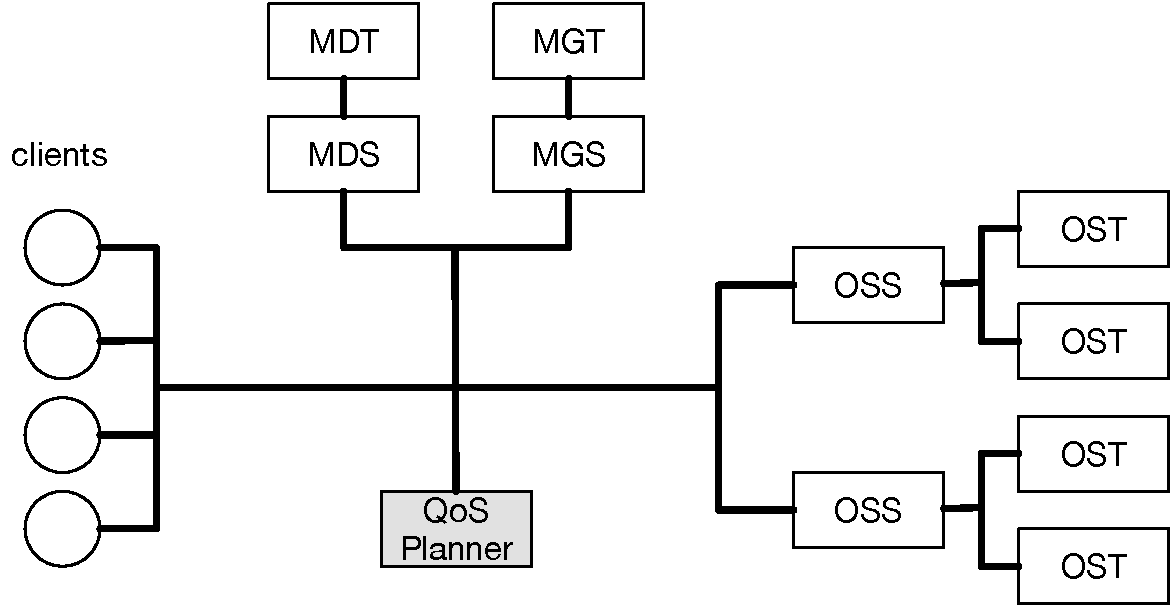
\includegraphics[width=.7\columnwidth]{figures/overview_system.pdf}
\label{subfig:global_view_lustre}
}\hfill
\subfloat[Key components and their relationship.]{
\centering
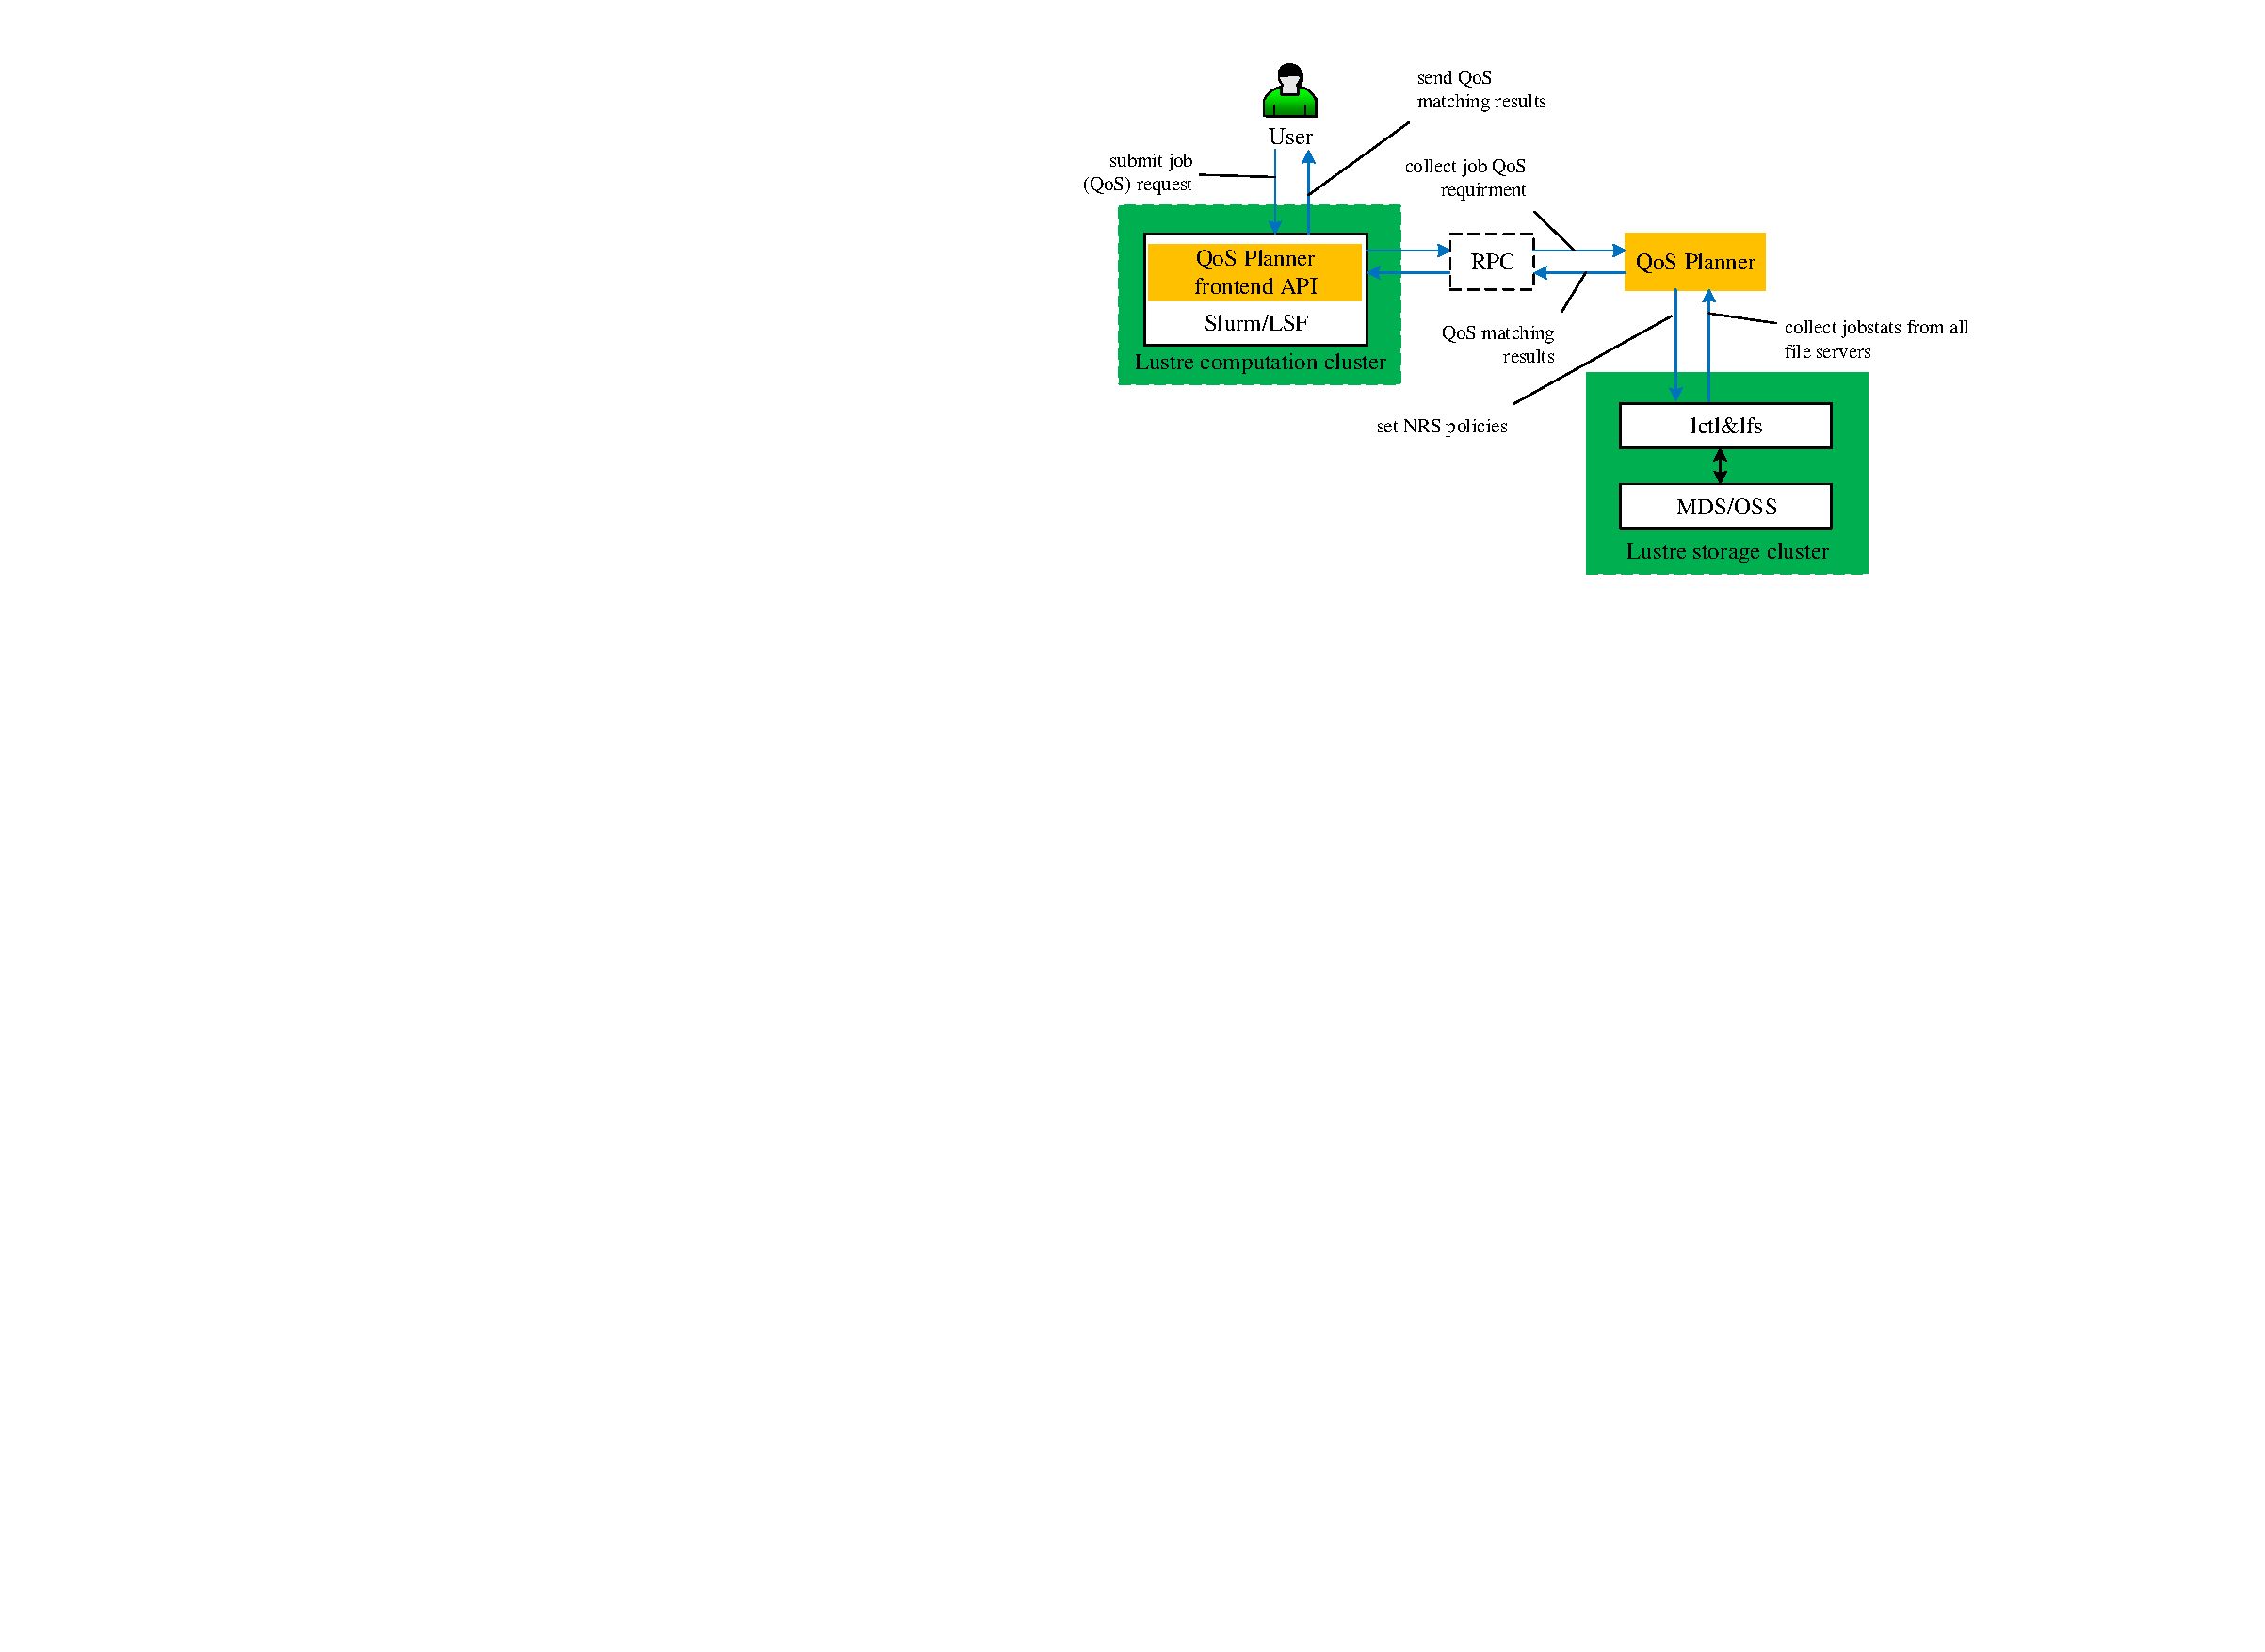
\includegraphics[width=.9\columnwidth]{figures/components_communication.pdf}
\label{subfig:qos_key_comp}
}\\
\subfloat[Communication steps.]{
\centering
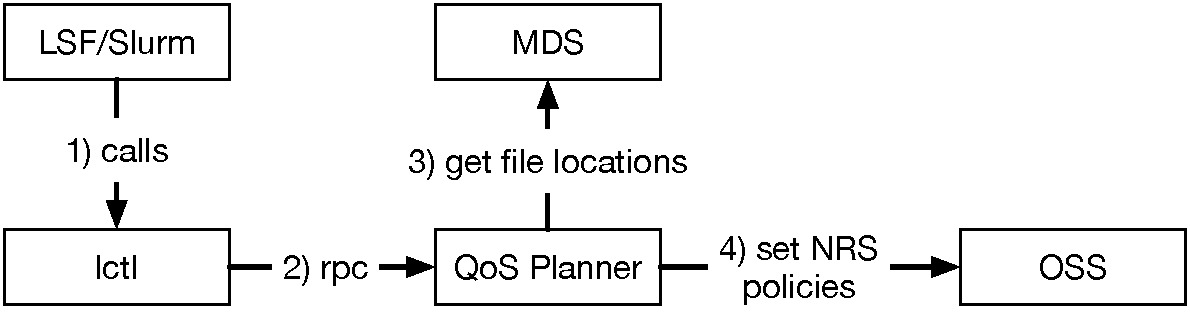
\includegraphics[width=.8\columnwidth]{figures/communication_flow.pdf}
\label{subfig:qos_comm_flow}
}
\caption{Overview.}
\label{fig:overview_system}
\end{figure}

\section{Software Architecture \& Related Libraries/Tools}
\subsection{Software architecture}
\begin{figure}[!ht]
\centering
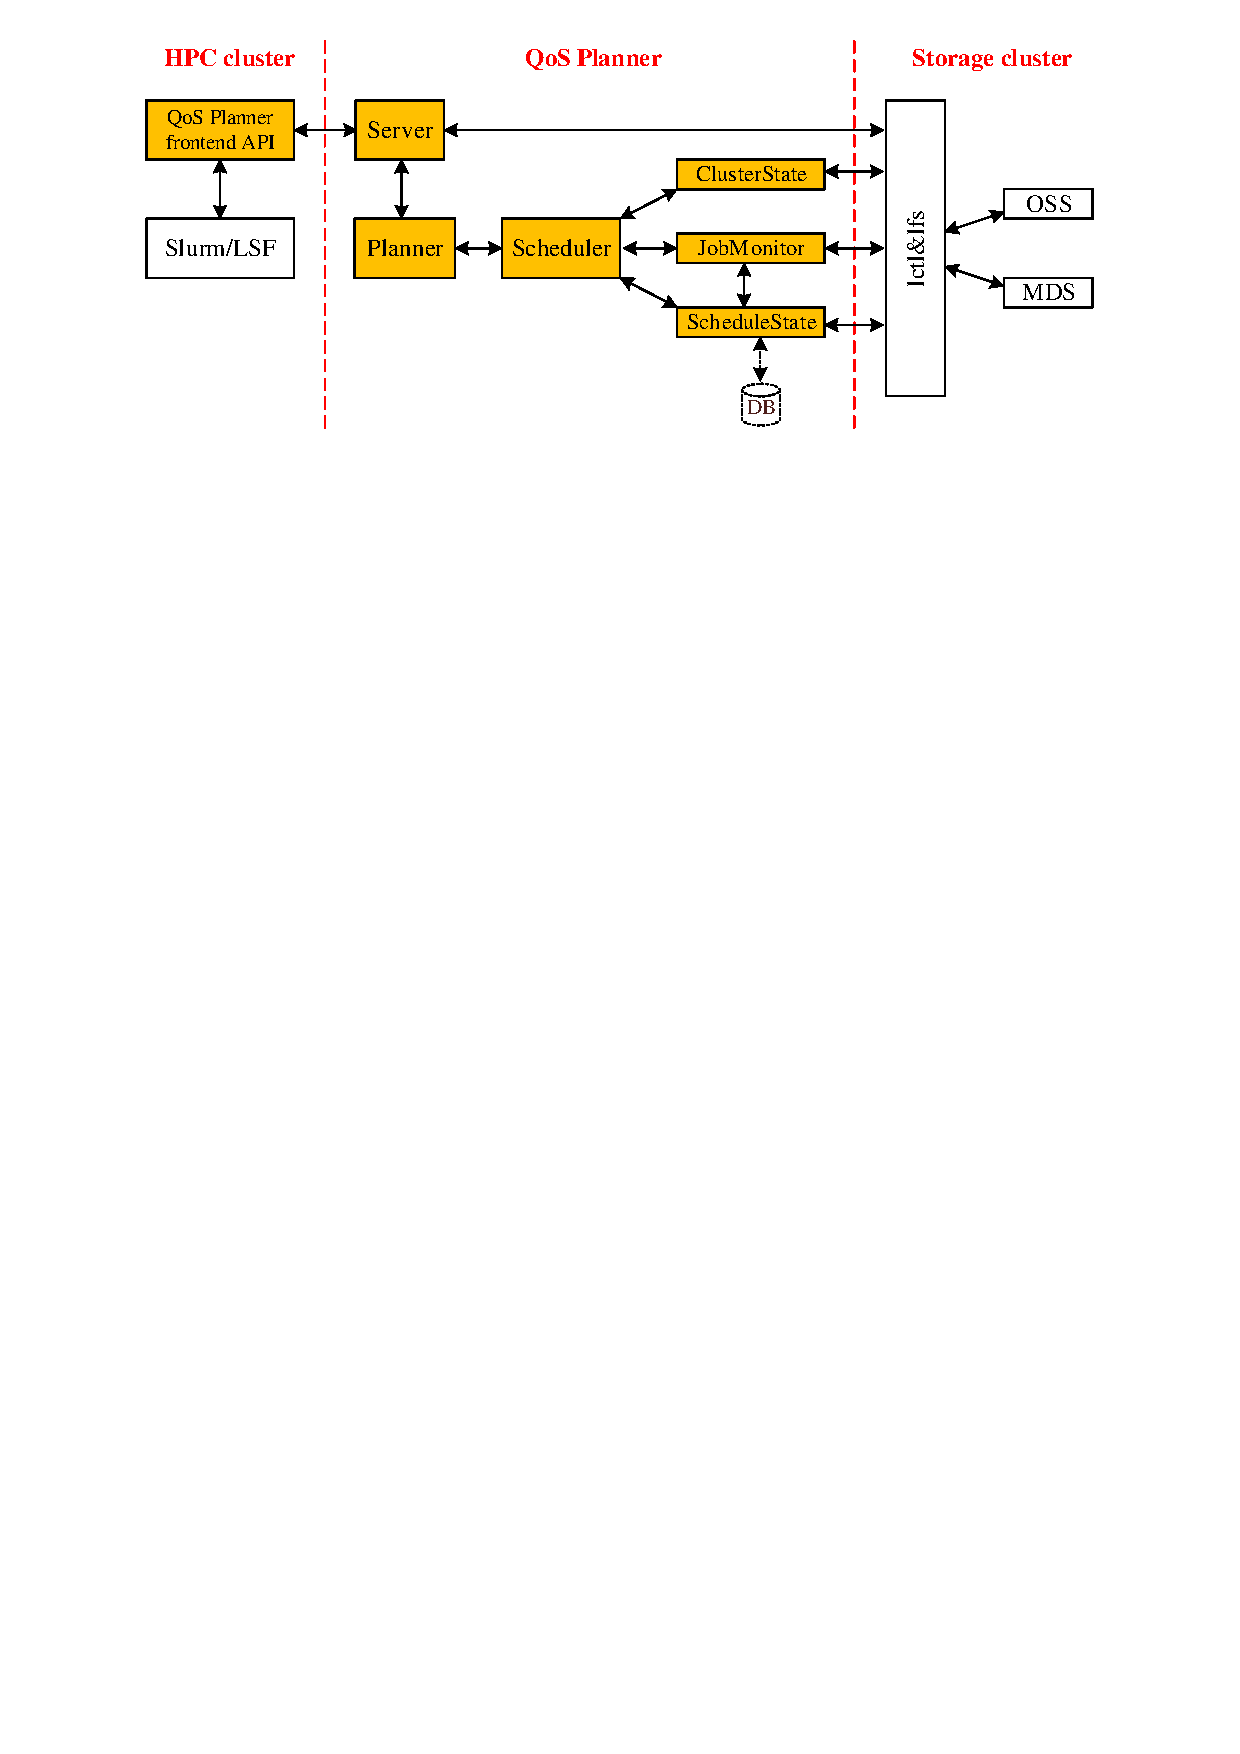
\includegraphics[width=.8\columnwidth]{figures/software_architecture_overview.pdf}
\caption{Software Architecture Overview.}
\label{fig:swarc_overview}
\end{figure}


Figure \ref{fig:swarc_overview} shows the overview of system software architecture in details. The whole system software architecture is composed of three parts, marked as HPC cluster, QoS Planner, and Storage cluster respectively (connecting via high performance network).

\textbf{HPC cluster}: This part includes all the computation nodes (or clients of Lustre). The Slurm/LSF is used as a workload manager for the HPC cluster. The Slurm/LSF can allocate exclusive and/or non-exclusive access to resources (HPC cluster) to users for some duration of time so they can perform work. Also the Slurm/LSF provides a framework for starting, executing, and monitoring job and arbitrates contention for resources by managing a queue of pending job. In our solution, we require to extend the \emph{lctl} in the Slurm/LSF. The \emph{QoS Planner frontend API} is used to communicate with the \emph{Server} in the QoS Planner.

\textbf{QoS Planner}: The modules of \emph{QoS Planner} includes:

(\textbf{{\romannumeral 1}}) The \emph{Server} module communicates with the \emph{QoS Planner frontend API} in the HPC cluster and gets OST information by the \emph{lctl\&lfs} utilities of the Lustre file system.

(\textbf{{\romannumeral 2}})  The \emph{Planner} module is in charge of the supply-and-demand issue for the scheduling job QoS. It provides the state of the \emph{Storage cluster} and sets the NRS according the QoS requirement (if the upply-and-demand is matching).

(\textbf{{\romannumeral 3}}) The \emph{Scheduler} module contains the scheduling algorithm. It reads the schedule when checking a job request and updates the schedule. The Scheduler also registers accepted jobs to the JobMonitor.
%(\textbf{{\romannumeral 3}}) The \emph{Scheduler} module collects the state of both the Storage cluster (by the \emph{ClusterState} module) and the scheduling state (by the \emph{ScheduleState} module). Also, the \emph{Scheduler} module monitors the job state in the Storage cluster by the \emph{JobMonitor} module.

(\textbf{{\romannumeral 4}}) The \emph{ClusterState} module collects the Storage cluster state (including network). This includes the set of OSS/OSTs as well as the current workload per OSS/OST.

(\textbf{{\romannumeral 5}}) The \emph{ScheduleState} module collects the Storage cluster scheduling state.

(\textbf{{\romannumeral 6}}) The \emph{JobMonitor} module ensures that Lustre is configured according to the schedule. New jobs mus be registered before they are considered.

\textbf{Storage cluster}: This part is a storage cluster managed by the Lustre file system.

%
\subsection{Related libraries/tools}
%
\subsubsection{ZeroMQ}
%
The ZeroMQ is used as a filter that collects data from some different remote publishers and sends it to local subscribers. The QoS Planner uses this library for the communication between the modified \emph{lclt} and itself.

\subsubsection{Protobuf}
We uses protocol buffers (a.k.a Protobuf) to implement automatic encoding and parsing of data with a binary format. It is also used for the communication between the modified \emph{lclt} and the QoS Planner.

\subsubsection{GFlags}
GFlags is used as a library to help parse the \emph{lctl} commandline and store the flags in some data structure.

\subsubsection{Cmake}
CMake is used to control the compilation process using simple platform and compiler independent configuration files, and to generate native makefiles and workspaces that can be used in the compiler environment of c++.

\subsubsection{GCC}
The GNU Compiler Collection (GCC) is used to compile C++ programming language.

\subsubsection{SSH}
Secure Shell (or SSH) is used to allow remote login and other network services by remote command-line login and remote command execution.

%%%%%%%%%%%%%%%%%%%%%%%%%%%%%%%%%%%%%%%%%%%%%%%%%%%%%
%%%%%%%%%%%%%%%%%%%%% Interface %%%%%%%%%%%%%%%%%%%%%
%%%%%%%%%%%%%%%%%%%%%%%%%%%%%%%%%%%%%%%%%%%%%%%%%%%%%
\section{Interface}

As mentioned in Section \ref{sect:general_design}, besides the new \textbf{QoS Planner}, we see interface changes both in the Slurm/LSF and in the Lustre file system.
The following subsections describe the minimal set of functions/changes.
We are going to extend the APIs gradually as we implement new features.

\subsection{HPC cluster side tool}
On the HPC cluster side, the job scheduling system (e.g. Slurm/LSF) must communicate with the QoS Planner to implement the resource reservation function.
It does so calling a cmdline tool by RPC, which can be a newly created tool or an extended version of \texttt{lctl}.
The HPC cluster side tool only acts as a frontend for the QoS Planner.
It directly forwards each request to the QoS Planner.

We identify the following basic operations.
Note that names etc.\ are preliminary and are open for discussion.

%%%%%%%%%%%%%%%%%%%%%%%%%%%%%%%%%%%%%%%%%%%%%%%%%%%%%
%%%%%%%%%%%%%%%%%%%%% RPC calls %%%%%%%%%%%%%%%%%%%%%
%%%%%%%%%%%%%%%%%%%%%%%%%%%%%%%%%%%%%%%%%%%%%%%%%%%%%

\begin{description}

\item[(1) reserve\_resources(JOBID, resource\_constraints, T$_{end})$]~\\ Asks the QoS Planner to reserve the given resources at the given time.
\begin{description}
    \item[Parameters]~\\
        \begin{description}
            \item[JOBID] Same job identifier as provided by LSF/Slurm.
            \item[resource\_constraints] list of resource constraints.
            The constraint for each file is given in the tuple $\langle file, Tp, T_{start}, T_{end}\rangle$.
            In the beginning, we focus on read intensive workloads, therefore this parameter should only be given for main input files for computations.
            This excludes small files such as shared libraries, for example.

            Note that the constraints for write throughput skip the $file$ parameter because the output files usually are created during the computation.
            %Note that the constraints also include timestamps and durations per file.
            While it might not be necessary for read-only files, specifying an interval $[T_{start}, T_{end}]$ becomes necessary when the QoS Planner also considers write throughput.
            It is hard to specify exact times for normal output files, but it is easy for checkpoints as they be triggered at scheduled times in some cases.
            Therefore, the HPC job only requires a short reservation of write throughput at different times.
            \item[$T_{end}$] The scheduled stop date of the job.
        \end{description}
    \item[Returns]~\\
        \begin{description}
            \item[0] OK
            \item[-1] not enough resources
            \item[-2] invalid args
        \end{description}
  \end{description}


\item[(2) free(JOBID)]~\\ Removes the reservation of resources for the given job.
  \begin{description}
    \item[Parameters]~\\
        \begin{description}
            \item[JOBID] Same identifier as giving when reserving resources. %LSF/Slurm
        \end{description}
    \item[Returns]~\\
        \begin{description}
            \item[0] OK
            \item[-1] error
        \end{description}
  \end{description}


\item[(3) ls\_jobs()]~\\ Convenience function. Lists all active resource reservations.
  \begin{description}
    \item[Parameters] no input necessary
    \item[Returns] list of active resource reservations
  \end{description}
\end{description}


\subsection{QoS Planner -- relating to OSS/NRS}
So far, users and administrators can set NRS rules only OSS-wide, i.e.\ the same NRS rules are applied to all OSTs belonging to the same OSS.
However, the QoS Planner needs to set NRS rule per OST.
Therefore, the existing API of NRS and \texttt{lctl} must be extended.

\subsection{QoS Planner -- relating to MDS}
In the third step in Figure \ref{subfig:qos_comm_flow}, the QoS Planner requests location information for a given file of the MDS.
So far, we have not found an existing RPC call for this task.

\begin{description}
\item[(1) get\_file\_locations(file)]~\\ Lists the OSTs which hold objects of the given file.
  \begin{description}
    \item[Parameters]~\\
        \begin{description}
            \item[file] The file identifier.
        \end{description}
    \item[Returns] lists the OSTs which hold objects of the given file.
  \end{description}
\end{description}



%%%%%%%%%%%%%%%%%%%%%%%%%%%%%%%%%%%%%%%%%%%%%%%%%%%%%
%%%%%%%%%%%%%%%%%%%% Open Issues %%%%%%%%%%%%%%%%%%%%
%%%%%%%%%%%%%%%%%%%%%%%%%%%%%%%%%%%%%%%%%%%%%%%%%%%%%
\section{Open Issues}

\begin{description}
 \item[Allow alternative schedules?] To reduce try-and-error cycles of LSF/Slurm, the QoS Planner could schedule requests at alternative times if wished and the original request cannot be met.

 \item[QoS Planner vs. normal NRS settings] QoS also can be configured via the \texttt{lctl} tool.
 This can overwrite rules set by the QoS Planner, thus destroying the schedule.
 Currently, the QoS Planner is designed with the assumption that he alone has control over the QoS configuration.
 How to solve this conflict?

 \item[QoS Planner as optional instance?] Is the planer an optional instance or a mandatory one?
 If the former: how to discover it?
 Add an entry to the MGS and let LSF/Lustre request the MGS regularly?
% TODO: clients müssen den QoS planer auch _entdecken_
% -> Eintrag in MGS?
% --> das hieße ein (initialer) zusätzlicher Kommunikationsschritt mit dem MGS. Das Wissen über den QoSPlanner kann dann in den clients vorgehalten werden.
% --> wie den QoSPlanner entdecken? Entweder direkt beim client-init oder später. "Später": a) per direkten announcment an alle clients b) per piggyback c) ???
% --> das Problem ist, dass es in Lustre noch nicht das Konzept von _optionalen_ Instanzen gibt, die dann nachträglich zugeschaltet werden können. Zugeschaltet werden können weitere OSS/OSTs, aber die werden implizit beim I/O entdeckt und sind nicht optional per Definition. Vielleicht wäre eine Lösung, den QoS als mandantory anzusehen und erst zu startetn, wenn der auch online ist?
\end{description}


%%%%%%%%%%%%%%%%%%%%%%%%%%%%%%%%%%%%%%%%%%%%%%%%%%%%%
%%%%%%%%%%%%%%%%%%%% Open Issues %%%%%%%%%%%%%%%%%%%%
%%%%%%%%%%%%%%%%%%%%%%%%%%%%%%%%%%%%%%%%%%%%%%%%%%%%%
\section{Future Work}

\begin{description}
 \item[Consider write throughput] So far, only read throughput is considered. As first extension, the QoS Planner also could consider write throughput.
 \item[Add real monitoring data] So far, static resource usage is assumed. In a later stage, it might be interesting to consider real workload data in the scheduling process.
\end{description}

\end{document}
